\documentclass{article}
\usepackage[margin=1.1in]{geometry}
\usepackage{graphicx}
\usepackage{amsmath}
\usepackage{amssymb}
\usepackage{hyperref}
\usepackage{booktabs}
\usepackage{xcolor}
\usepackage{listings}
\usepackage{tcolorbox}
\usepackage{pdfpages}
\tcbuselibrary{listings, skins, breakable}

% Output box environment (black background, white text)
\newtcolorbox{outputbox}[1]{
    arc=3mm,
    boxrule=1pt,
    colback=black!85!white,
    colframe=black,
    coltext=white,
    title={\textbf{#1}},
    fontupper=\ttfamily\scriptsize,
    left=2mm, right=2mm, top=2mm, bottom=2mm,
    fontupper=\ttfamily\scriptsize\obeylines,
    breakable
}

% Python code box environment
\lstdefinestyle{pythonstyle}{
    language=Python,
    basicstyle=\ttfamily\scriptsize,
    keywordstyle=\color{blue!80!black}\bfseries,
    stringstyle=\color{green!60!black},
    commentstyle=\color{gray}\itshape,
    showstringspaces=false,
    numbers=left,
    numberstyle=\tiny\color{gray},
    numbersep=3.5pt,
    breaklines=true,
    tabsize=4
}
\newtcblisting{pythonbox}[1]{
    arc=3mm,
    boxrule=1pt,
    colback=yellow!5!white,
    colframe=yellow!50!black,
    title={\textbf{#1}},
    listing only,
    listing style=pythonstyle,
    breakable
}

% ── Title ─────────────────────────────────────────────────────────────────────
\begin{document}

\begin{titlepage}
\begin{center}


\includegraphics[width=0.55\textwidth]{images/ozu.png}\\[2cm]

\rule{\linewidth}{0.5mm}\\[0.4cm]

{ \LARGE
  \textbf{PHYS551: Advanced Monte Carlo Methods}\\[0.4cm]
  \emph{Homework 5}\\[0.4cm]
}
\rule{\linewidth}{0.5mm}\\[0.4cm]

\hfill\hfill

\linewidth=0.8\textwidth
\begin{minipage}{0.4\textwidth}
    \begin{flushleft} \large
        \emph{Student:}\\
        Ömer Faruk \textsc{Avcı}
    \end{flushleft}
\end{minipage}
~
\begin{minipage}{0.5\textwidth}
    \begin{flushright} \large
        \emph{Instructor:}\\
        Prof. Dr. Taylan \textsc{Akdo\u{g}an}\\[0.1cm]
    \end{flushright}
\end{minipage}

\vfill

\textsc{\large Department of Electrical and Electronics Engineering}\\[0.4cm]

{\large \today}

\end{center}
\end{titlepage}

\section*{Disclosures and References}

\textbf{AI Usage Disclosure:} In accordance with the course policy, I would like to declare the extent of AI assistance used in this assignment:

\begin{itemize}
    \item \textbf{Code \& Visualizations:} AI tools were utilized to assist in generating the output plots and to refine/add descriptive comments to the Python source code.
    \item \textbf{Document Preparation:} AI assistance was used to construct, format, and style the LaTeX document to ensure a clean and professional layout.
\end{itemize}

\newpage

% =============================================================
% PROBLEM 1
% =============================================================
\section*{Problem 1: The Underflow Trap}

\subsection*{Part (a): Mathematical Derivation}
The formal mathematical proof demonstrating the strict logical equivalence between the standard acceptance condition and the log-space condition is attached below.

% This command inserts your scanned PDF pages here
\begin{center}
    % Adjust the 0.9 up or down to scale your scanned image
    
\includegraphics[width=0.8\textwidth]{problem_1_derivation.pdf}
\end{center}

\subsection*{Part (b): Code Upgrade}
To prevent \texttt{NaN} crashes resulting from floating-point underflow, the target function has been upgraded to compute the natural logarithm of the probability directly. The \texttt{np.exp()} call was removed from the target function. The Metropolis-Hastings engine was subsequently modified to subtract log-probabilities (rather than dividing raw probabilities) and the acceptance check was updated to use $\ln(u) < \alpha$.

\begin{pythonbox}{Log-Space Metropolis-Hastings Engine}
def log_target_f(state):
    x, y = state
    # Upgraded: np.exp() removed to prevent underflow
    return -(x ** 2) / 20.0 - (y - (x ** 2) / 4.0) ** 2 / 2.0

def metropolis_hasting_log_space(num_steps, sigma, start_state):
    samples = np.zeros((num_steps, 2))
    accepted_moves = 0
    samples[0] = start_state
    current_state = start_state
    
    current_log_prob = log_target_f(current_state)

    for i in range(1, num_steps):
        proposal = current_state + np.random.normal(0, sigma, size=2)
        proposal_log_prob = log_target_f(proposal)

        # EVALUATE: Subtraction in log-space replaces division
        alpha = proposal_log_prob - current_log_prob

        # DECIDE: log(u) < alpha
        if np.log(np.random.uniform(0, 1)) < alpha:
            current_state = proposal
            current_log_prob = proposal_log_prob
            accepted_moves += 1

        samples[i] = current_state

    acceptance_rate = accepted_moves / (num_steps - 1)
    return samples, acceptance_rate
\end{pythonbox}

\newpage

% =============================================================
% PROBLEM 2
% =============================================================
\section*{Problem 2: Bayesian Parameter Estimation: The Exoplanet Hunt}

\subsection*{Part (a) \& (b): Algorithm Implementation and Tuning}
The target log-posterior function was constructed by combining the uniform prior constraints ($K \in [0, 30]$, $P \in [2, 12]$) with the Gaussian log-likelihood of the noisy telescope data. 

The Metropolis-Hastings algorithm was initialized at $K=5.0$, $P=5.0$ and run for $N=50,000$ steps. Because the amplitude ($K$) and period ($P$) operate on fundamentally different scales, a single step size $\sigma$ would result in highly inefficient mixing. To achieve an optimal acceptance rate, the proposal standard deviations were tuned independently to $\sigma_K = 2.5$ and $\sigma_P = 0.1$. This configuration successfully yielded an acceptance rate of $27.5\%$, placing the chain perfectly within the optimal $20\% - 40\%$ ``Goldilocks zone.''

\begin{pythonbox}{Log-Posterior Function}
def log_posterior(state):
    K, P = state
    
    # 1. Prior Constraints
    if not (0 <= K <= 30) or not (2 <= P <= 12):
        return -np.inf 
        
    # 2. Log-Likelihood Calculation
    predictions = K * np.sin((2 * np.pi / P) * t_days)
    log_likelihood = -0.5 * np.sum( ((v_obs - predictions) / sigma_noise)**2 )
    
    return log_likelihood
\end{pythonbox}

\subsection*{Part (c): Convergence and Burn-in Analysis}
As illustrated in the trace plots below, the chain exhibits rapid mixing after the initial traversal from the starting guess. The first $10,000$ iterations were discarded as burn-in to ensure the remaining samples represent the true stationary distribution.

\begin{figure}[h!]
    \centering
    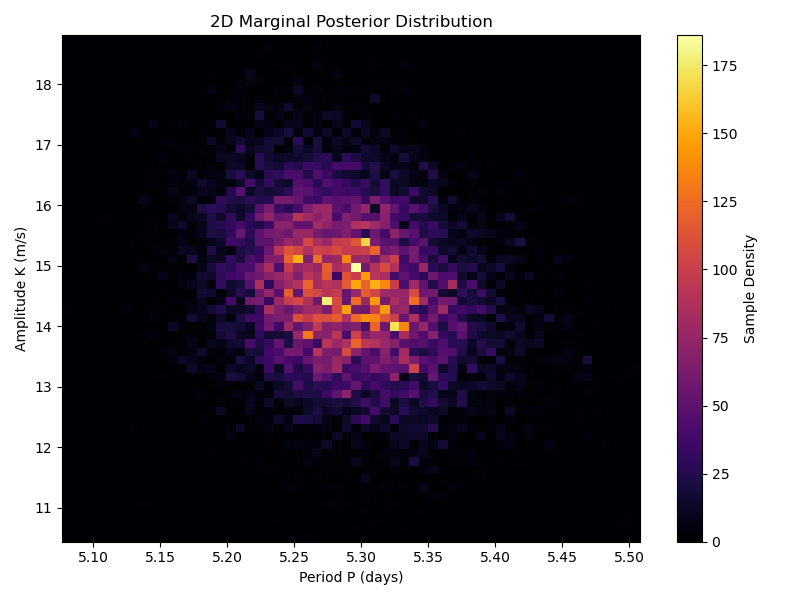
\includegraphics[width=0.8\textwidth]{images/problem_2_1_figure.png}
    \caption{Trace plot for Velocity Amplitude ($K$).}
\end{figure}


\begin{figure}[h!]
    \centering
    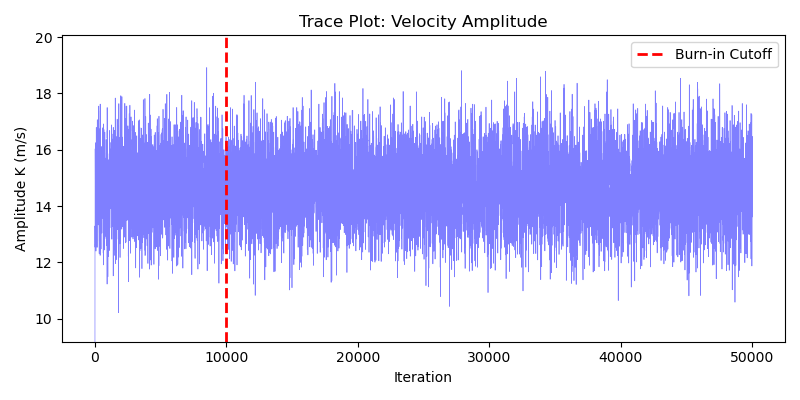
\includegraphics[width=0.8\textwidth]{images/problem_2_2_figure.png}
    \caption{Trace plot for Orbital Period ($P$).}
\end{figure}

\newpage
\subsection*{Part (d): Posterior Distribution and Parameter Estimates}

Following the removal of the burn-in phase, the remaining $40,000$ samples were used to approximate the posterior distribution and extract the physical parameters. The 2D histogram below demonstrates that the parameters are tightly constrained by the data, indicating a highly probable physical state.

\begin{figure}[h!]
    \centering
    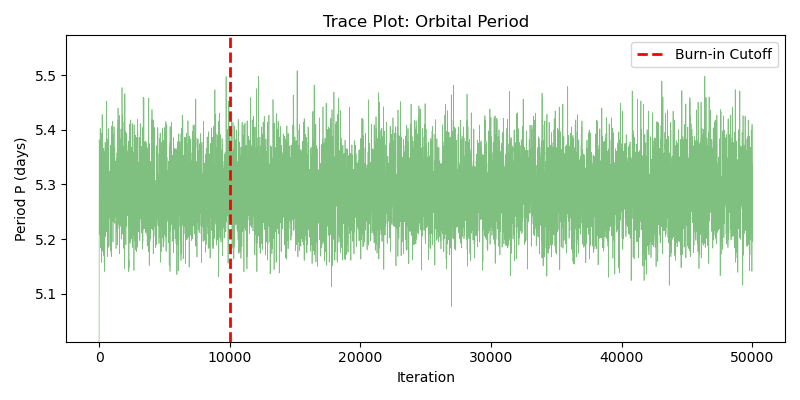
\includegraphics[width=0.75\textwidth]{images/problem_2_3_figure.png}
    \caption{2D Marginal Posterior Distribution of the Exoplanet Orbital Period and Velocity Amplitude.}
\end{figure}

Using the post-burn-in MCMC samples, the expected values and standard errors for the exoplanet parameters were calculated. The low variance in the period estimation indicates the telescope data is highly sensitive to the orbital frequency.

\begin{outputbox}{Final Parameter Estimates (MCMC Results)}
Acceptance Rate = 27.5%

Amplitude (K) = 14.66 ± 1.13 m/s
Period (P)    = 5.290 ± 0.052 days
\end{outputbox}

\begin{pythonbox}{Implementation of Problem 2}
"""

# PHYS 551: Advanced Monte Carlo Methods
# Homework 3 - Source Code
# Student: Omer Faruk Avci
# Instructor: Prof. Dr. Taylan Akdogan

"""
import numpy as np
import matplotlib.pyplot as plt

"""Problem 2: Bayesian Parameter Estimation: The Exoplanet Hunt"""

# Telescope observation data (Time, Velocity, and Measurement Noise)
days_t = np.array([1.2, 2.5, 3.1, 4.8, 6.5, 7.2, 8.1, 9.5, 10.3, 11.9])
v_obs = np.array([12.4, -4.5, -13.2, -6.1, 14.8, 11.2, -3.8, -14.9, -9.1, 13.5])
sigma_noise = 2.5

def v_model(t, K, P):
    # Theoretical radial velocity model (sine wave)
    return K * np.sin((2 * np.pi / P) * t)

def log_posterior(state):
    K, P = state

    # Enforce uniform prior constraints: K in [0, 30], P in [2, 12]
    if not (0 <= K <= 30 and 2 <= P <= 12):
        return -np.inf
    
    # Calculate predicted velocities using the current state parameters
    predicted = v_model(days_t, K, P)
    
    # Compute the log-likelihood assuming Gaussian noise
    log_likelihood = -0.5 * np.sum(((v_obs - predicted) / sigma_noise) ** 2)

    # Since the prior is uniform, posterior is proportional to likelihood
    return log_likelihood

def metropolis_hasting_2d(num_steps, sigmas, start_state):
    # Array to store all generated MCMC samples
    samples = np.zeros((num_steps, 2))
    accepted_moves = 0

    # Initialize the Markov chain
    current_state = start_state
    current_log_prob = log_posterior(current_state)
    samples[0] = current_state

    for i in range(1, num_steps):
        # Propose a new state using independent Gaussian jumps for K and P
        proposal = current_state + np.random.normal(0, sigmas)
        proposal_log_prob = log_posterior(proposal)

        # Calculate the acceptance ratio in log-space (subtraction replaces division)
        alpha = proposal_log_prob - current_log_prob

        # Accept or reject the jump based on a log-uniform random draw
        if np.log(np.random.uniform(0, 1)) < alpha:
            current_state = proposal
            current_log_prob = proposal_log_prob
            accepted_moves += 1

        # Record the state (either the newly accepted state or the old repeated state)
        samples[i] = current_state

    acceptance_rate = accepted_moves / (num_steps - 1)
    return samples, acceptance_rate

def main():
    num_steps = 50_000
    burn_in = 10_000
    start_point = np.array([5.0, 5.0])
    
    # TUNING: K gets a 1.5 jump, P gets a tiny 0.05 jump.
    sigmas = np.array([2.5, 0.1]) 

    print("Running MCMC Exoplanet Hunt...")
    samples, acc_rate = metropolis_hasting_2d(num_steps, sigmas, start_point)
    print(f"Acceptance Rate: {acc_rate * 100:.1f}%")

    # --- Analyze Valid Data (Discard Burn-in) ---
    # Slice the array to remove the initial unmixed samples
    valid_samples = samples[burn_in:]
    K_samples = valid_samples[:, 0]
    P_samples = valid_samples[:, 1]

    # Calculate final physical parameters (Mean +/- Std Dev)
    K_mean, K_std = np.mean(K_samples), np.std(K_samples)
    P_mean, P_std = np.mean(P_samples), np.std(P_samples)
    
    print("\nFinal Results:")
    print(f"Amplitude (K) = {K_mean:.2f} ± {K_std:.2f} m/s")
    print(f"Period (P)    = {P_mean:.3f} ± {P_std:.3f} days")

    # --- Plotting (Separate Figures) ---
    
    # Calculate tight Y-axis limits based only on the valid samples (ignoring burn-in)
    k_min, k_max = np.min(K_samples), np.max(K_samples)
    k_pad = (k_max - k_min) * 0.15 
    
    p_min, p_max = np.min(P_samples), np.max(P_samples)
    p_pad = (p_max - p_min) * 0.15

    # 1. Trace Plot for K
    plt.figure(figsize=(8, 4))
    plt.plot(samples[:, 0], color='blue', alpha=0.5, linewidth=0.5)
    plt.axvline(burn_in, color='red', linestyle='--', linewidth=2, label='Burn-in Cutoff')
    plt.ylim(k_min - k_pad, k_max + k_pad) # NARROWED Y-AXIS
    plt.ylabel('Amplitude K (m/s)')
    plt.xlabel('Iteration')
    plt.title('Trace Plot: Velocity Amplitude')
    plt.legend()
    plt.tight_layout()
    plt.savefig('trace_K.png')
    plt.show()

    plt.close() # Closes the figure so it doesn't overlap with the next one

    # 2. Trace Plot for P
    plt.figure(figsize=(8, 4))
    plt.plot(samples[:, 1], color='green', alpha=0.5, linewidth=0.5)
    plt.axvline(burn_in, color='red', linestyle='--', linewidth=2, label='Burn-in Cutoff')
    plt.ylim(p_min - p_pad, p_max + p_pad) # NARROWED Y-AXIS
    plt.ylabel('Period P (days)')
    plt.xlabel('Iteration')
    plt.title('Trace Plot: Orbital Period')
    plt.legend()
    plt.tight_layout()
    plt.savefig('trace_P.png')
    plt.show()

    plt.close()

    # 3. 2D Posterior Scatter / Histogram
    plt.figure(figsize=(8, 6))
    h = plt.hist2d(P_samples, K_samples, bins=60, cmap='inferno')
    plt.colorbar(h[3], label='Sample Density')
    plt.xlabel('Period P (days)')
    plt.ylabel('Amplitude K (m/s)')
    plt.title('2D Marginal Posterior Distribution')
    plt.tight_layout()
    plt.savefig('posterior_2d.png')
    
    plt.show()

if __name__ == "__main__":
    main()
\end{pythonbox}

\end{document}